\chapter[Perturbation for ODE]{Regular Perturbation methods for ODEs}
This is the heart of the course. The ``regular'' theory is the ``vanilla'' variant. To understand, consider the projectile problem

\paragraph{Example 1:} Launch a toy rocket straight up. How long does it take to hit the ground if $g$ is varying with height $x$ above the Earth's surface?
\begin{align}
	\cancel{m} \ddot{x} &= -\frac{GM\cancel{m}}{(R+x)^2} = -\frac{GM}{R^2} \frac{R^2}{(R+x)^2} \nonumber \\
	&= -g \frac{R^2}{(R+x)^2} \label{eqn:wk11-rocket}
\end{align}
The initial conditions are
\begin{align*}
	x(0) &= 0 \\
	\dot{x}(0) &= v_0
\end{align*}
Assume initial velocity is small such that $x \ll R$ for all $t$. Na\"{i}vely
\begin{gather}
	\ddot{x} \approx -g \nonumber \\
	x(t) \approx  -\frac{1}{2}gt^2 + v_0 t \label{eqn:wk11-rocket-approx}
\end{gather}
What is the leading correction to this solution? It is better to scale the problem and work with dimensionless units: the characteristic time $t_c$ is, say, the time it takes to reach the peak and the characteristic scale $x_c$ is the peak height. Ignoring any $O(1)$ factor, we see
\begin{gather*}
	t_c = \frac{v_0}{g} \qquad x_c = \frac{v_0^2}{g}
\end{gather*}
and introduce the new dimensionless variables
\begin{gather*}
	\tau = \frac{t}{t_c} \qquad y = \frac{x}{x_c}
\end{gather*}
In terms of these our governing eqn. \ref{eqn:wk11-rocket} reads:
\begin{gather*}
	\frac{\md^2 y}{\md \tau^2} = - \frac{1}{\left(1 + \dfrac{x_c y}{R}\right)^2}
\end{gather*}
Defining $x_c/R = \epsilon $ we arrive at the form
\begin{gather*}
	y'' = -\frac{1}{(1+\epsilon y)^2}
\end{gather*}
The parameter
\begin{gather*}
	\epsilon = \frac{v_0^2}{gR} \ll 1
\end{gather*}
also suggests that the initial velocity is much smaller than the escape velocity. The initial conditions now read
\begin{align*}
	y(0) &= \frac{x(0)}{x_c} = 0 \\
	y'(0) &= \frac{t_c}{x_c} \dot{x}(0) = 1
\end{align*}
In summary, we are left to solve the nonlinear ODE subject to the BCs
\begin{gather}
	y'' = -\frac{1}{(1+ \epsilon y)^2}, \qquad 
	y(0) = 0, \qquad y'(0) = 1 \label{eqn:wk11-example1-ode}
\end{gather}
We try the solution which is a power series in $\epsilon$
\begin{gather}
	y(\tau,\epsilon) = y_0(\tau) + \epsilon y_1(\tau) + \epsilon^2 y_2(\tau) + \dots \label{eqn:wk11-soln-ansatz}
\end{gather}
with our IC reading
\begin{align*}
	\underbrace{y(0,\epsilon)}_0 &= y_0(0) + \epsilon y_1(0) + \dots = 0 + 0 \epsilon + \dots \\
	\underbrace{y'(0,\epsilon)}_1 &= y_0'(0) + \epsilon y'_1(0) + \dots = 1 + 0 \epsilon + \dots 
\end{align*}
Inserting our ansatz -- eqn. \ref{eqn:wk11-soln-ansatz} -- into the ODE:
\begin{align*}
	y_0'' + \epsilon y_1'' + \dots &= -(1+ \epsilon y)^{-2} \\
	&= -1 + 2\epsilon y + O(\epsilon^2) \\
	&= -1 + 2\epsilon y_0 + \dots 
\end{align*}
Our hierarchy of equations read:
\begin{align*}
	O(\epsilon^0) &: \quad y_0'' = -1 \\
	O(\epsilon^1) &: \quad y_1'' = 2y_0
\end{align*}
Solving the $O(1)$ equation:
\begin{gather*}
	y_0(\tau) = -\frac{1}{2}\tau^2 + \tau 
\end{gather*}
which is simply the dimensionless version of eqn. \ref{eqn:wk11-rocket-approx}. The $O(\epsilon^1)$ equation gives us the leading order correction to this:
\begin{gather*}
	y_1(\tau) = -\frac{1}{12} \tau^4 + \frac{1}{3} \tau^3
\end{gather*}
Pulling everything together
\begin{gather}
	y(\tau,\epsilon) = \tau -\frac{\tau^2}{2} + \epsilon \left(\frac{\tau^3}{3} - \frac{\tau^4}{12}\right) + \dots \label{eqn:wk11-rocket-correction}
\end{gather}
Now in our dimensionless variables, the time it takes for the rocket to return is simply when $y(\tau)=0$, which yields
\begin{gather*}
	\tau = 0 \qquad \tau = 2
\end{gather*}
What is the time it takes for the rocket to hit the ground when the leading order correction given by eqn. \ref{eqn:wk11-rocket-correction} is considered? We must now solve the algebraic equation 
\begin{align*}
	0 = \tau -\frac{\tau^2}{2} + \epsilon \left(\frac{\tau^3}{3} - \frac{\tau^4}{12}\right)
\end{align*}
which we attempt to solve with the solution form, following sec. \ref{sec:pert-algebra} ex. 1
\begin{gather*}
	\tau^\ast = 2 + \epsilon \tau^\ast_1 + O(\epsilon^2)
\end{gather*}
Then, neglecting $O(\epsilon^2)$ terms
\begin{gather*}
	0 = (2+\epsilon \tau_1^\ast) - \frac{1}{2}(4+ 4\epsilon \tau_1^\ast) + \epsilon \left[\frac{1}{3}(8+12\epsilon \tau_1^\ast)-\frac{1}{12}(16+32 \epsilon \tau_1^\ast)\right]
\end{gather*}
which yields $\tau_1^\ast = 4/3$ and
\begin{gather*}
	\tau = 2 + \frac{4}{3}\epsilon + \dots 
\end{gather*}
\begin{figure}[!h]
	\centering
	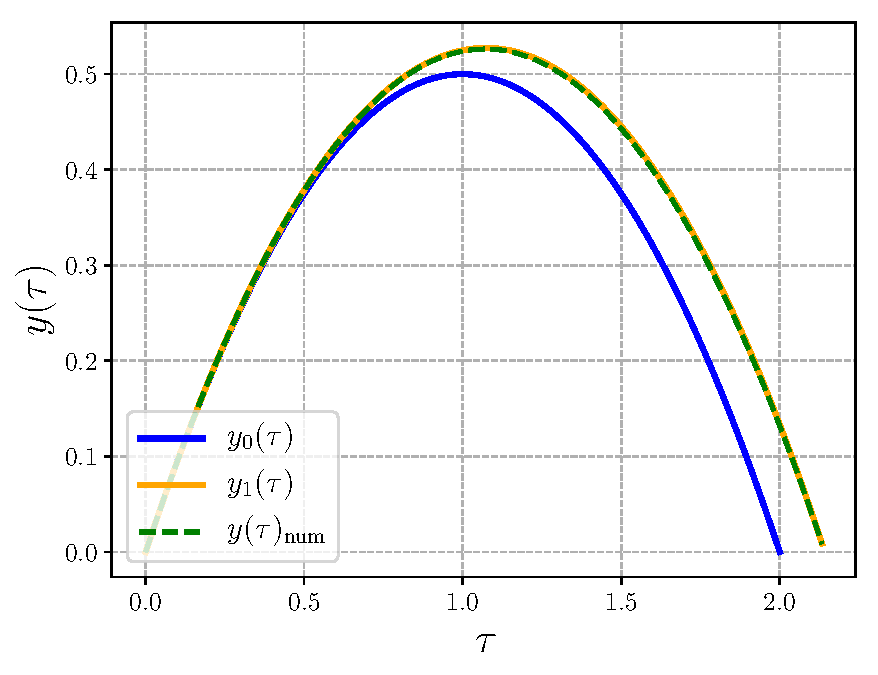
\includegraphics[width=0.65\textwidth]{./plots/pdf/strogatz-wk11.pdf}
	\caption{Plotting the numerical solution to eqn. \ref{eqn:wk11-example1-ode} along with the analytical approximations given by eqn. \ref{eqn:wk11-rocket-correction} for $\epsilon=0.1$. The numerical and higher order solutions have been plotted to $\tau = 2 + 4\epsilon/3$, which is the corrected time it takes for the projectile to hit the ground.}
	\label{fig:strogatz-wk11}
\end{figure} \\

\paragraph{Example 2:} Solve
\begin{gather*}
	y' + y + \epsilon y^2 = 0
\end{gather*}
with the IC $y(0)=1$ on the interval $[0,\infty)$ ignoring $O(\epsilon^2)$. We try a regular perturbation series
\begin{gather*}
	y(x,\epsilon) = y_0(x) + \epsilon y_1(x) + O(\epsilon^2)
\end{gather*}
The ICs translate to
\begin{gather*}
	y(0,\epsilon) = 1 + 0\epsilon + \dots = y_0 + \epsilon y_1 + \dots 
\end{gather*}
and our ODE becomes
\begin{gather*}
	(y_0' + \epsilon y_1' + \dots) + (y_0 + \epsilon y_1 + \dots ) + \epsilon (y_0 + \epsilon y_1 + \dots)^2 = 0
\end{gather*}
which yields the hierarchy of equations
\begin{align*}
	O(\epsilon^0): \qquad & y_0' + y_0 = 0\\
	O(\epsilon^1): \qquad & y_1' + y_1 + y_0^2 = 0 
\end{align*}
Solving these sequentially:
\begin{gather*}
	y_0(x) = \me^{-x}
\end{gather*}
and
\begin{gather*}
	y_1' + y_1 = -\me^{-2x}
\end{gather*}
Such first order ODEs can be straightforwardly solved using the integrating factor method. This yields
\begin{gather*}
	y_1(x) = -\me^{-x} + \me^{-2x}
\end{gather*}
and our solution
\begin{gather}\label{eqn:wk11-ex2-pertsoln}
	y(x,\epsilon) = \me^{-x} + \epsilon (-\me^{-x} + \me^{-2x})
\end{gather}
Now our contrived example can be solved exactly by writing as
\begin{gather*}
	\int \left[\frac{1}{y} - \frac{\epsilon}{1+\epsilon y}\right] \md y = -x + c
\end{gather*}
which with the proper boundary condition yields
\begin{gather*}
	\ln \left[\frac{y}{1+\epsilon y} (1+\epsilon)\right] = -x 
\end{gather*}
Some rearrangement yields
\begin{gather}\label{eqn:wk11-ex2-exactsoln}
	y(x,\epsilon) = \frac{1}{-\epsilon + (1+\epsilon)\me^x}
\end{gather}
In the complex $\epsilon$ plane, the function $y(x,\epsilon)$ \underline{converges for all $x$} with the radius of convergence $R(x)$\footnote{$R(x)$ is the distance from the origin to the nearest singularity of $y(x,\epsilon)$.} when
\begin{gather*}
	-\epsilon + (1+\epsilon)\me^x = 0 \\
	\epsilon_\mathrm{singular} = \frac{\me^x}{1 - \me^x}
\end{gather*}
Observe that for \underline{any} $x \geq 0$
\begin{gather*}
	|\epsilon_\mathrm{singular}| = \left| \frac{\me^x}{\me^x-1} \right| > 1
\end{gather*}
i.e. $|\epsilon|<1$ ensures convergence for \underline{all} $x$. Refer to the solution plots in Fig. \ref{fig:strogatz-wk11-ex2}. The perturbative solution matches well over the full domain in $x$ -- this is referred to as ``uniform approximation/validity''. This feature typifies ``regular'' perturbation problems.
\begin{figure}[!h]
	\centering
	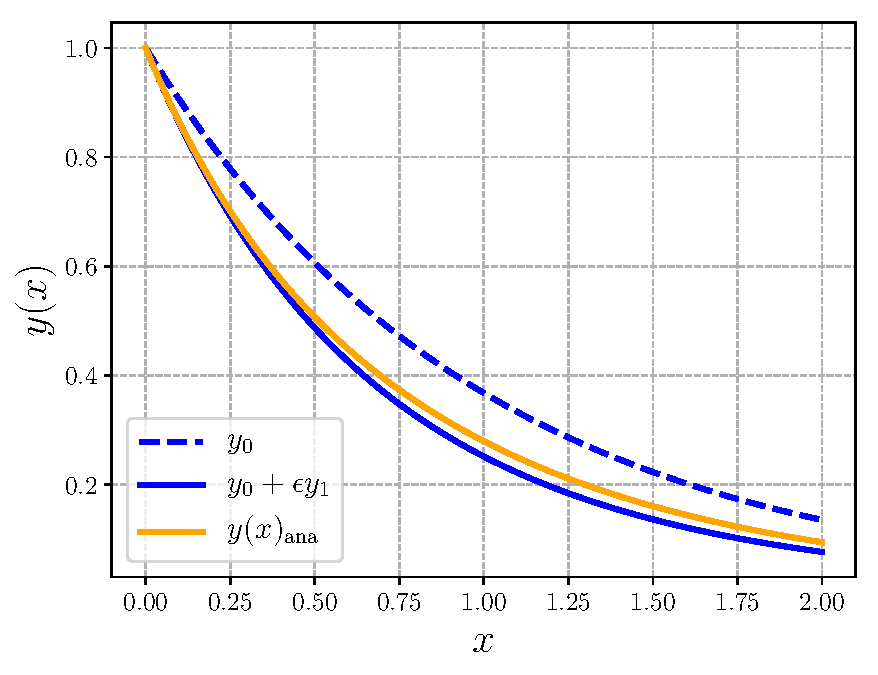
\includegraphics[width=0.65\textwidth]{./plots/pdf/strogatz-wk11-ex2.pdf}
	\caption{The exact soln. \ref{eqn:wk11-ex2-exactsoln} and perturbative soln. \ref{eqn:wk11-ex2-pertsoln} plotted for $\epsilon = 0.5$.}
	\label{fig:strogatz-wk11-ex2}
\end{figure}

\paragraph{Example 3:} However, there are bad $x$. So our solution is asymptotic, but not uniformly valid. Consider
\begin{gather*}
	f(x,\epsilon) = x + \me^{-x/\epsilon}
\end{gather*}
where $x \in (0,1)$. As $\epsilon \rightarrow 0^+$
\begin{gather*}
	f(x)\sim x
\end{gather*}
and further the dropped term is a TST. Despite this, as can be seen from Fig. \ref{fig:strogatz-wk11-ex3}, the approximate solution is not uniformly valid. 
\begin{figure}[!h]
	\centering
	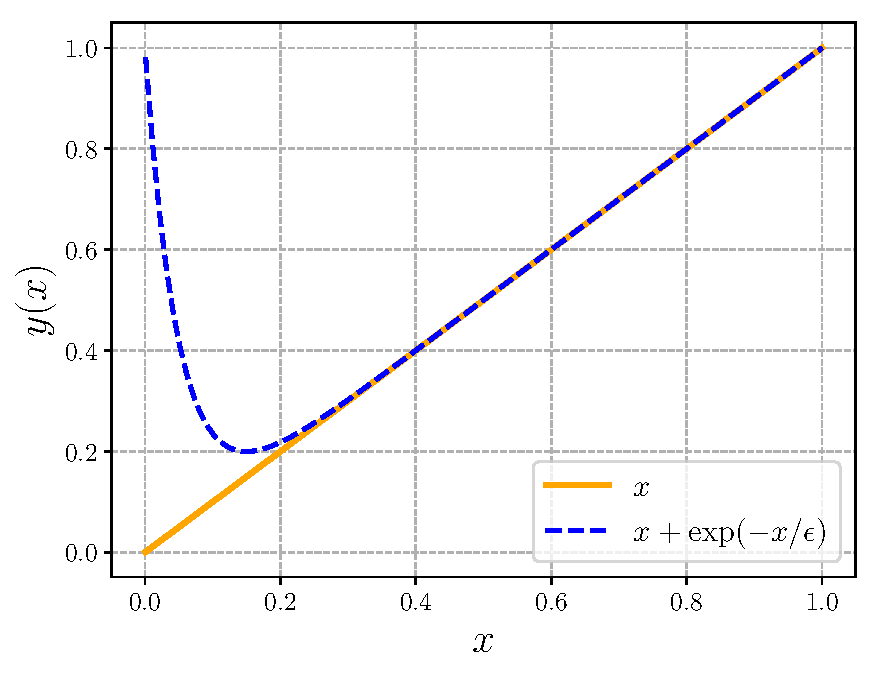
\includegraphics[width=0.65\textwidth]{./plots/pdf/strogatz-wk11-ex3.pdf}
	\caption{$f(x,\epsilon)$ and $f(x)\sim x$ plotted for $\epsilon = 0.05$.}
	\label{fig:strogatz-wk11-ex3}
\end{figure} \\
When this kind of phenomenon happens, we have a ``boundary layer'' and are very important in fluid dynamics.
